\documentclass[../thesis.tex]{subfiles}
\begin{document}
\chapter{Applied Integrated Lifetimes}\label{sec:decoupling_applications}

Chapter \ref{sec:integrated_lifetime} discussed a novel approach for decoupling lifetime.  
The studies in this chapter use this technique and exploit this additional information to better understand device behavior.
This includes a discussions of \textcite{Hershey2017} in Section \ref{sec:cbp_host}, \textcite{Bangsund2018} in Section \ref{sec:lifetime_meml}, and \textcite{Bangsund2018a} in Section \ref{sec:lifetime_dow}, as well as unpublished work.


\section{CBP Host Thickness}\label{sec:cbp_host}

\subsection{Motivation and Experimental}

%\begin{wrapfigure}{r}{.4\textwidth}
\begin{figure}[ht]
\centering
\begin{subfigure}{.3\textwidth}
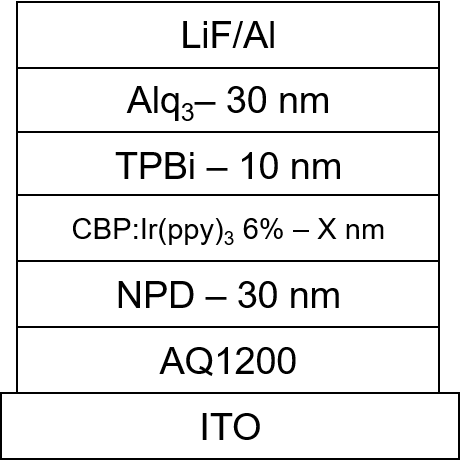
\includegraphics[width=\textwidth]{lifetimeApplications/architecture}
\caption{}
\label{fig:cbp_architecture}
\end{subfigure}
\begin{subfigure}{.4\textwidth}
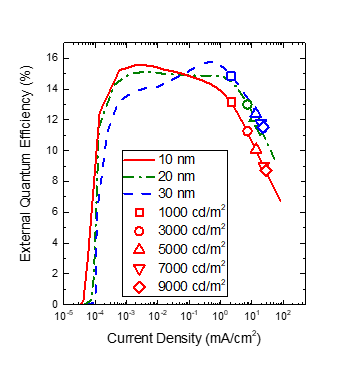
\includegraphics[width=\textwidth]{lifetimeApplications/eqe}
\caption{}
\label{fig:cbp_eqe}
\end{subfigure}
\caption{a. Device architecture, featuring EML thicknesses of X=10,20, and 30 nm.  b. External Quantum Efficiency ($\eta_{EQE}$) for the three architectures.  Operational points for lifetime are shown in symbols.}
\end{figure}


Carbazole materials are architypical hosts for phosphorescent devices, most common among them being 4,4'-Bis(N-carbazolyly)-1,1'-biphenyl (CBP).\supercite{Han2014,OBrien1999a,Cho2014,Price2015,Adachi2001,Watanabe2007,Holmes2003,Adamovich2003}
Therefore, CBP was used as a preliminary system to demonstrate the decoupling technique.
Devices consisted of a 40-nm-thick hole-injection layer of Plexcore AQ1200 spun-cast on a glass substrate coated with a 150-nm-thick layer of  indium-tin-oxide (ITO), followed by a 30-nm-thick hole-transport layer of N,N' -Bis(naphthalen-1-yl)-N,N' -bis(phenyl)-benzidine (NPD), and an EML of 4,4'-Bis(N-carbazolyl)-1,1'-biphenyl (CBP) doped at 6 vol. % with tris[2-phenylpyridinato-C2,N]iridium(III) (Ir(ppy)3).  The emissive layer was capped with a 10-nm-thick layer of 2,2′,2"-(1,3,5-Benzinetriyl)-tris(1-phenyl-1-H-benzimidazole) (TPBi), and a 30-nm-thick layer of tris-(8-hydroxyquinoline)aluminum (Alq3). The cathode for each device consisted of a 0.5-nm-thick layer of LiF and a 100-nm-thick layer of Al.
All devices were fabricated according to the processes outlined in Chapter \ref{sec:oleds_fabrication}.
The structure shown in Figure \ref{fig:cbp_architecture} was used with EML thicknesses of X=10, 20, and 30 nm.
The \eqe for all three EML thicknesses, shown in Figure \ref{fig:cbp_eqe}, shows maximum efficiencies of 15.7\%, 15.3\%, and 15.7\% for EML thicknesses of 10, 20, 30 nm, respectively.
Though similar in peak value, as thicknesses increases, the peak \eqe shifts to higher current.
This is indicative of a shift in the charge dynamics and possible location of the recombination zone.
Recombination zone has been previously linked with lifetime, with a longer lifetime expected for thicker RZ.\supercite{Zhang2014,Wu2016,Chin2005,Lee2006,Chwang2002,Han2016,Lee2005a,Brown2004,Choong2000,Liu2004}
Using an ambipolar host such as CBP, one would expect that expanding the EML would result in a wider RZ and thus longer lifetime.

\subsection{Results}

\begin{figure}[ht]
\centering
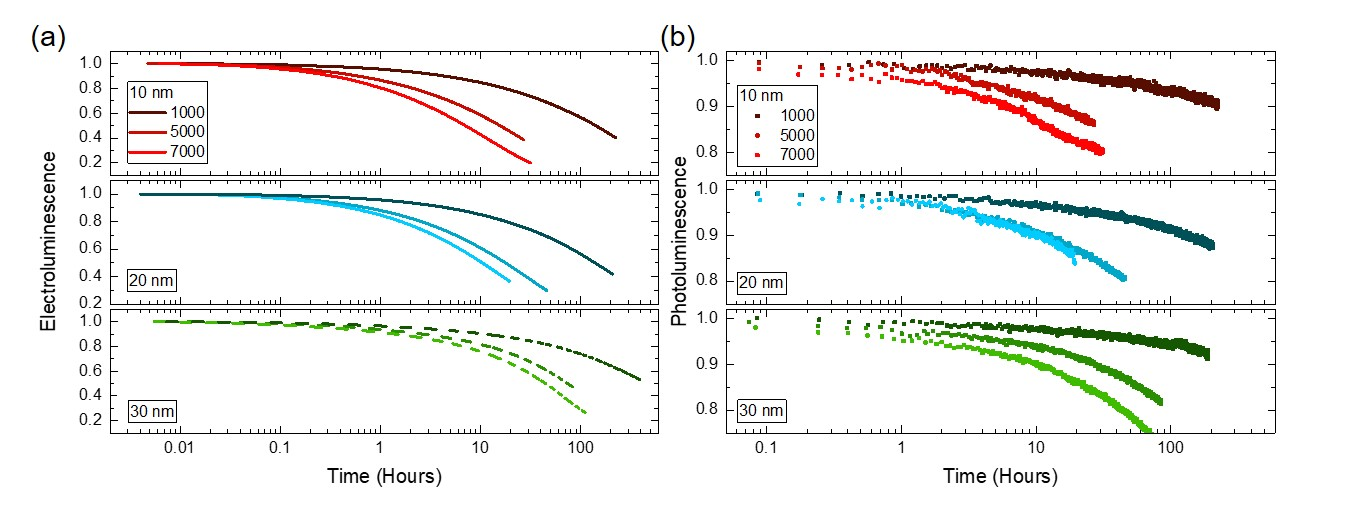
\includegraphics[width=\textwidth]{lifetimeApplications/elpl}
\caption{Device decay curves for multiple values of the initial luminance as a function of emissive layer thickness.  Loss in (a) electroluminescence (EL) and (b) photoluminescence (PL) are shown and decrease monotonically with increasing luminance.  For devices with a 10-nm-thick emissive layer, initial luminance values are 1000 $cd/m^2$, 5000 $cd/m^2$, and 7000 $cd/m^2$.  For devices with a 20-nm- or 30-nm-thick emissive layer, initial luminance values are 1000 $cd/m^2$, 5000 $cd/m^2$, and 7100 $cd/m^2$. }
\label{fig:cbp_elpl}
\end{figure}

Figure \ref{fig:cbp_elpl}a shows the traditional EL lifetimes of these devices, and indeed the 30 nm EML shows a longer lifetime than the 10 and 20 nm.  
In Figure \ref{fig:cbp_elpl}b, the intermittent \pl measurements can be seen, showing the advantage of this technique and the large amount of additional data that is available.
The operational conditions of each device is shown in Table \ref{tab:lifetime_summary}.
Similar currents are used across EML thicknesses, but voltage increases slightly with thickness, as might be expected.

\begin{table}[hb]
\centering
\begin{tabular}{c|c|c|c|c}
$d_{EML}$ (nm) & $L_0$ (cd/m$^2$) & $J$ (mA/cm$^2$) & $V_0$ (V) & $t_{50}$ (hours) \\
\hline
& 1000 & 2.2 & 4.2 & 139.0 \\
& 3000 & 7.2 & 5.1 & 39.9 \\
10 & 5000 & 13.6 & 5.4 & 15.8 \\
& 7000 & 14.4 & 6.2 & 6.9 \\
& 9000 & 28.0 &  6.3 & 5.3 \\
\hline
& 1000 & 2.2 & 5.4 & 141.1 \\
& 3000 & 7.2 & 6.0 & 33.1 \\
20 & 5000 & 12.4 & 7.2 & 17.2 \\
& 7100 & 19.2 & 7.3 & 10.0 \\
& 9000 & 24.0 &  7.5 & 8.0 \\
\hline
& 1000 & 2.2 & 5.9 & 474 \\
30 & 5000 & 13.6 & 7.3 & 74.4\\
& 7100 & 19.6 & 7.6 & 46 \\
& 8000 & 22.4 &  7.7 & 38.1 \\

\end{tabular}
\caption{Summary of device lifetimes.  For each device, the starting luminance ($L_0$), current density ($J$), starting voltage ($V_0$) and time at which 50\% of the initial luminance is reached ($t_{50}$) are reported.}
\label{tab:lifetime_summary}
\end{table}

To be able to extract \pl and \ef, \oc and $\chi$ cannot change during degradation.
No birefringence was observed under cross polarization before or after degradation, suggesting the absence of large-scale crystallization which would change \oc .  
No new emission features are observed with degradation, suggesting that the emissive state is unchanged and $\chi$ can be assumed constant.
With these assumptions satisfied, \pl and \ef can be extracted from the measured PL intensity, and are shown in Figure \ref{fig:tx_components}.



\begin{wrapfigure}{r}{.6\textwidth}
\centering
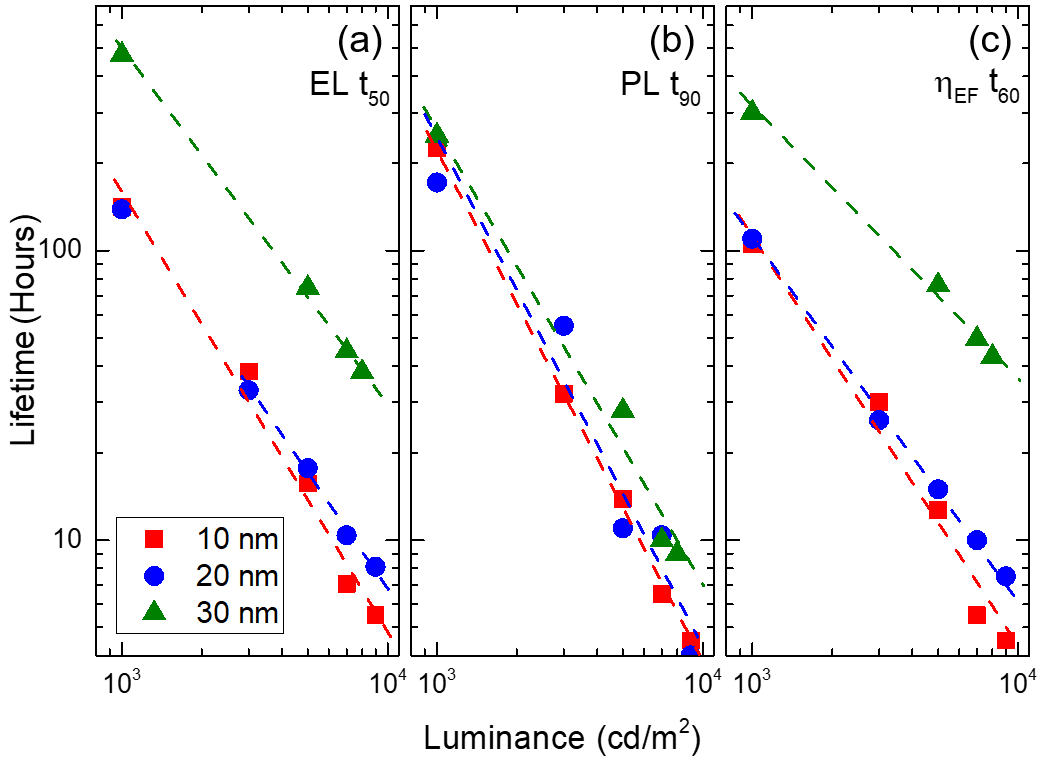
\includegraphics[width=0.6\textwidth]{lifetimeApplications/tx_components}
\caption{Extracted lifetimes for all 3 architectures as a function of luminance.}
\label{fig:tx_components}
\end{wrapfigure}

The lifetime decreases with luminance for all architectures.  
While a reduction in the EL lifetime is observed in Figures \ref{fig:cbp_elpl} and \ref{fig:tx_components} in reducing device thickness from 30 nm to 20 nm, little difference is seen between devices having EML thicknesses of 20 nm and 10 nm.  
The degradation in the PL intensity does not appear to be a strong function of EML thickness.  
Indeed, comparing the EL and PL lifetimes with the extracted degradation in exciton formation shows that the EL decay is dominated by a loss in the efficiency of exciton formation with \ef reaching 60\% of its initial value by the time EL has reached 50\%.  
A substantial component of this decay is likely due to non-radiative recombination center formation.\supercite{Kondakov2003,Kondakov2007d}
Over this same period, the PL intensity has only degraded by ~10\% of its initial value.

The similarity in PL degradation observed across all EML thicknesses suggests that the exciton and polaron densities are similar between these devices,\supercite{Giebink2008a,Coburn2017,Lee2017} thus have similar exciton recombination zone widths.  
The accelerated degradation in the exciton formation efficiency (\ef) observed for devices with EML thicknesses of 10 nm and 20 nm suggests that the recombination zone samples the EML/TPBi interface, which has been previously shown to cause degradation.\supercite{Wang2013,Wang2014}
This change in recombination zone location is also suggested by the \eqe behavior shifting peak location, shown in Figure \ref{fig:cbp_eqe}.
To validate this suggestion, the position of the recombination zone was assessed in the devices with EML thickness of 20 and 30 nm devices using a quenching TPTBP sensitizer.  
The position of the recombination zone can be inferred by the corresponding reduction in device \eqe due to quenching by TPTBP.\supercite{Erickson2013a}
The sensitized 30-nm-thick EML devices showed no quenching, suggesting no recombination near the interface, while devices with a 20-nm-thick EML showed quenching only at the EML/TPBi interface, confirming the position of the recombination zone at that interface.  
Devices with a 10-nm-thick EML exhibited changing current-voltage behavior when sensitized with TPTBP, and thus PtTPTBP, an emissive sensitizer with a peak wavelength of 770 nm, was used in 2-nm-thick strips on either side of the EML at 0.5 vol. \%.
This configuration was able to match the current-voltage behavior of the control device while permitting the measurement of emission from PtTPTBP.  
For devices with a 10-nm-thick EML, strong emission from PtTPTBP is observed from the EML/TPBi interface and weak emission seen from the EML/NPD interface. 
These quenching experiments are shown in Figure \ref{fig:cbp_rz}.
These results suggest that for devices with an EML thickness of 10 nm or 20 nm, the recombination zone samples the EML/TPBi interface, accelerating exciton formation loss.  
While detailed analysis of the relevant degradation mechanism is the subject of future work, previous work has suggested a role played by exciton-polaron interactions.\supercite{Wang2015a,Zhang2016,Giebink2008a,Kondakov2007d,Kondakov2003}

\begin{figure}[hb]
\centering
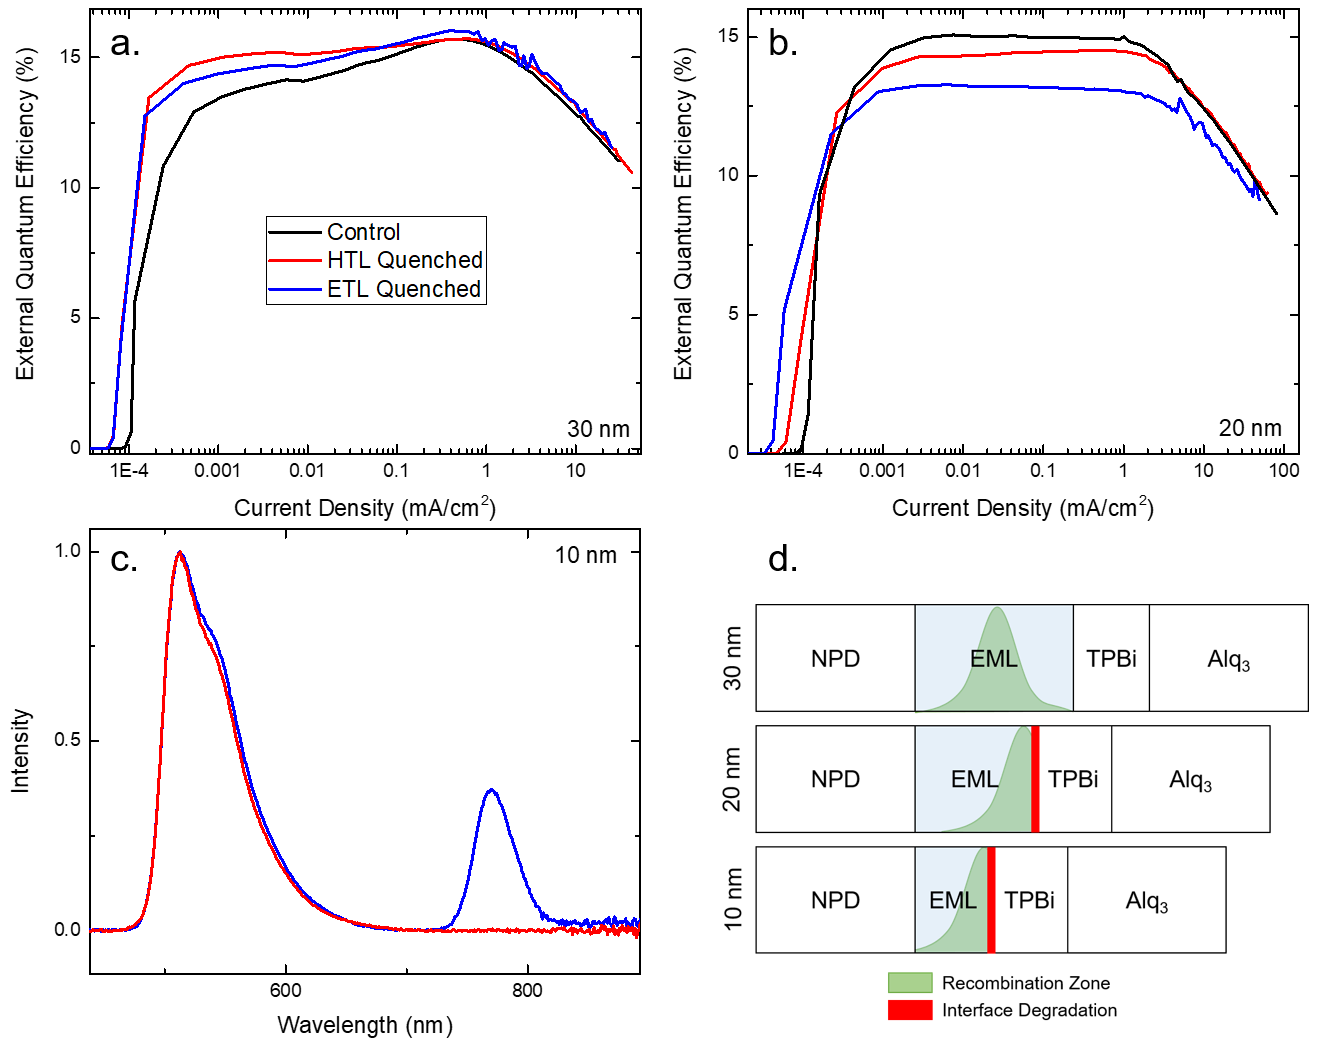
\includegraphics[width=.8\textwidth]{lifetimeApplications/cbp_rz}
\caption{a. TPTBP quenched 30 nm devices.  No quenching is observed.  b. TPTBP quenched 20 nm devices.  Quenching is observed for the ETL side quencher, and minimally for the HTL side. c. PtTPTBP quenched 10 nm EML devices. Emission from the sensitizer only at the ETL. d. Summary of recombination zone measurements.}
\label{fig:cbp_rz}
\end{figure}

\subsection{Conclusion}

The additional information offered by this technique is directed at improving the screening of active materials and device architectures for the realization of long-lived OLEDs.  
Device degradation that is dominated by a loss in either \ef  or \pl implies a dominant rate process and an opportunity for improvement of materials or architecture.  
In systems using \irppy, a relatively stable emitter with demonstrated long optical and electrical lifetimes,\supercite{Scholz2015} losses in the exciton formation efficiency are expected to represent the majority fraction of degradation.  
However, for novel molecules, limiting processes are largely unknown and would benefit from the separation of emitter and exciton formation efficiency loss.  
PL degradation could become increasingly important for blue-emitting species where the high exciton energies could contribute to material degradation.  \supercite{Scholz2015,Xu2016,Coburn2016a,Lee2015,Yi2016,Kim2008}
This screening process would be dramatically improved if \ef and \pl can be mechanistically modeled.  
With additional datasets, modeling and understanding of degradation mechanisms can be improved and help to identify limiting processes.
The model presented in \textcite{Giebink2008a} could easily be adapted to seperate losses that would be captured by \pl and \ef, and would provide further checks to this overparameterized model.

In summary, this work presents a method for decoupling optical and electrical losses during OLED operational decay by attributing the overall reduction in electroluminescence to a loss in \pl or the exciton formation efficiency through \ef.  
Model devices are shown as a function of luminance, with a loss in \ef shown to be the limiting factor for the short-lived devices.  
By measuring the recombination zone, these devices are shown to be subject to interfacial degradation, only seen in narrow EML devices.
Contrary to the expectation, the RZ is not found to expand with the EML thickness, but rather to shift within the device.
This technique allows access to additional experimental information which can offer insight about the degradation mechanism and understanding of device luminance loss.  
This added information can be used to aid future efforts in modeling degradation.

\section{MEML Luminance Scaling}\label{sec:lifetime_meml}

\begin{wrapfigure}{r}{.4\textwidth}
\centering
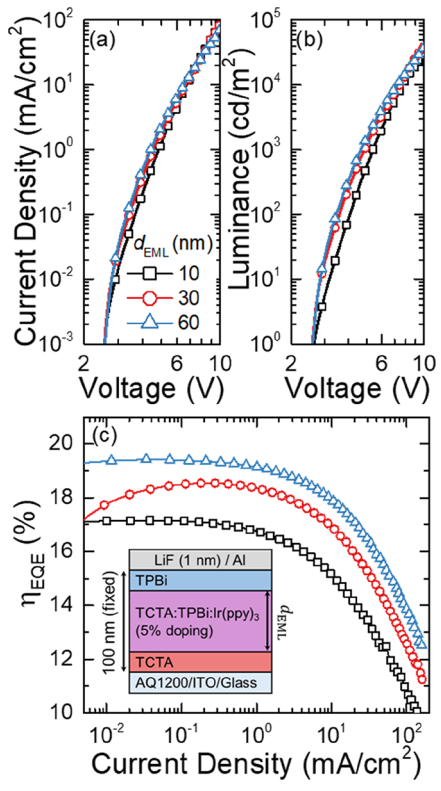
\includegraphics[width=.3\textwidth]{lifetimeApplications/meml_eqe}
\caption{a. Current Density and b. Luminance as a function of Voltage.  c. \eqe for all three EML thicknesses.  Inset is MEML device architecture.}
\label{fig:meml_eqe}
\end{wrapfigure}

This section outlines the work done in \textcite{Bangsund2018a}.  
All figures are reproduced from this work, while the text is an adapted version of the paper text.

\subsection{Motivation}

As discussed in Section \ref{sec:cbp_host}, recombination zone width has been extensively connected with lifetime, mediated by the exciton and polaron populations.\supercite{Scholz2015,Giebink2008a,Giebink2009a,So2010,Zhang2016,Schmidbauer2013,Wu2016,Lee2006,Chwang2002}
However, despite this observed trend with recombination zone thickness, the specific role of the RZ in degradation kinetics is still an active area of investigation.
Using a mixed emmissive layer (MEML) architecture, this works seeks to provide a more concrete connection between the recombination zone and degradation within the same system.  

\subsection{Experimental}

\begin{wrapfigure}{r}{.4\textwidth}
\centering
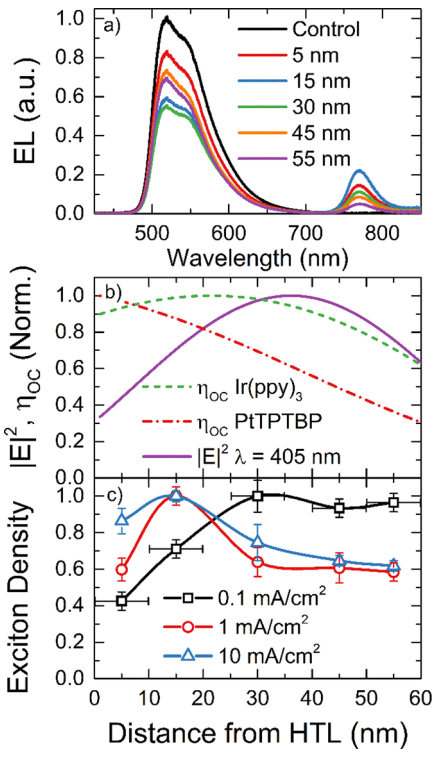
\includegraphics[width=.4\textwidth]{lifetimeApplications/meml_rz}
\caption{a. Raw spectra of sensitized devices.  b. Out-coupling for \irppy and PtTPTBP across the EML as well as electric field profille.  c. RZ as a function of current density.  For all currents, the RZ is found to span the entire EML.}
\label{fig:meml_rz}
\end{wrapfigure}

Devices consisted of a 60-nm-thick hole injection layer (HIL) of poly(thiophene-3-[2[(2-methoxyethoxy)ethoxy]-2,5-diyl)(AQ1200, Sigma Aldrich), a 4,4',4"-tris(N-carbazolyl)triphenylamine (TCTA, TCI America) hole-transport layer (HTL), a mixed-host emissive layer (M-EML) consisting of a 47.5 vol.% TCTA, 47.5 vol.% 2,2',2''(1,3,5-benzenetriyl) tris-(1-phenyl-1H-benzimidazole) (TPBi, Lumtec) and 5 vol.% of the green phosphorescent emitter fac-tris(2-phenylpyridine)iridium(III) (Ir(ppy)3, Lumtec), a TPBi electron-transport layer (ETL), and a LiF (1 nm)/Al (100 nm) cathode. 
All layers were deposited according to the procedures outlined in Section \ref{sec:oleds_fabrication}.
When varying the M-EML thickness (10 nm, 30 nm, 60 nm), the HTL and ETL thicknesses are varied equally to maintain a total device thickness of 100 nm.
Device characteristics are shown in Figure \ref{fig:meml_eqe}, with the efficiency increasing slightly from 17\% to 19\% as the EML thickness increases from 10 to 60 nm.

This device architecture system, shown in the inset of Figure \ref{fig:meml_eqe}, was chosen because of its broad recombination zone, which spans the entire EML.\supercite{Erickson2013a}
Because of this property, the MEML thicknes, $d_{eml}$ can be taken as a proxy for the RZ width, and the exciton density can be controlled by modifying the EML.
The increase in recombination zone thickness is evidenced by the change in onset of the roll-off with increasing RZ width, seen in Figure \ref{fig:meml_eqe}c.


To experimentally confirm the RZ breadth, the 60 nm EML architecture was investigated using PtTPTBP as a sensitizer, using the methodology outlined in Chapter \ref{sec:rz_measurement}.
The exciton density is found to remain above 60\% of the peak across the entire 60 nm M-EML at a current density of 10 mA/cm$^2$, shown in Figure \ref{fig:meml_rz}. 
As current density increases from 0.1 mA/cm2 to 10 mA/cm2, the peak of the RZ migrates from the ETL side to the HTL side of the M-EML. 
These findings are consistent with other reports for similar device architectures,\supercite{Erickson2013a} and confirm that $d_{eml}$ is a good proxy for RZ width.
The 60 nm EML is the thickest investigated EML thickness and should be subject to the most variation in RZ intensity accross the EML.  
Therefore, thinner EML devices are also assumed to have a RZ spanning the EML.

\subsection{Results}

\begin{wrapfigure}{r}{.4\textwidth}
\centering
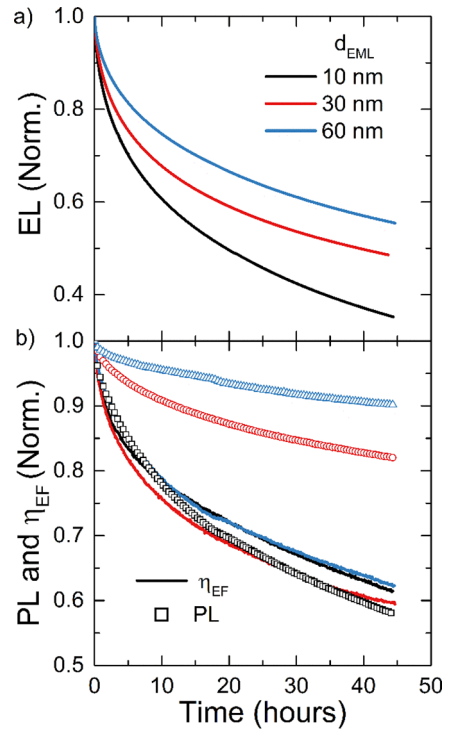
\includegraphics[width=.4\textwidth]{lifetimeApplications/meml_lifetime}
\caption{a. EL lifetime at 3,000 cd/m$^2$ for EML thicknesses of 10,30,60 nm.  b. The corresponding \pl and \ef degradation.}
\label{fig:meml_lifetime}
\end{wrapfigure}

The degradation of these devices at a initial luminance of $L_0$=3,000 cd/m$^2$ is shown in Figure \ref{fig:meml_lifetime}a.
The EL lifetime increases by approximately a factor of 3 in increasing the thickness from 10 nm to 60 nm, and nearly all this enhancement can be attributed to a reduced rate of PL degradation, shown in Figure \ref{fig:meml_lifetime}b.
No trend with thickness is apparent in the \ef decays, which are all within typical device-to-device variation. 
In contrast, the PL decays show a dramatic separation with thickness. 
We also note that a reduction in \ef dominates the overall degradation rate in the 30 nm and 60 nm thick M-EML devices, but is comparable to PL losses in the 10 nm M-EML device. 
These results suggest that reduced degradation in emissive layer PL efficiency may be the primary reason for enhanced stability in M-EML architectures, as compared to with their single-host counterparts. 
Moreover, the combination of improved efficiency roll-off and PL lifetime with an increased RZ width, and thus decreased exciton density, provides further evidence of a link between bimolecular annihilation events and the degradation of PL efficiency. \supercite{Schmidbauer2013}
Losses in \ef, however, appear to be relatively insensitive to exciton density.

\begin{wrapfigure}{r}{.4\textwidth}
\centering
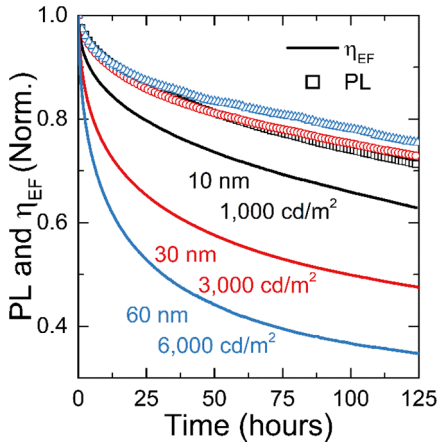
\includegraphics[width=.4\textwidth]{lifetimeApplications/meml_scaled_lifetime}
\caption{Lifetimes of devices with luminance scaled to match the EML thickness. PL collapses due to matched exciton density.}
\label{fig:meml_scaled_lifetime}
\end{wrapfigure}

To show that exciton density and PL loss are intimately related, the exciton density was matched between the architectures by scaling the luminance to the EML thickness ratio.  
The 10, 30, and 60 nm EML devices were operated at initial luminances of 1,000, 3,000, and 6,000 cd/m$^2$, respectively.
The results of this aging are shown in Figure \ref{fig:meml_scaled_lifetime}.
PL degradation is nearly identical for 10, 30, and 60 nm M-EML devices operated at luminances of 1,000, 3,000, and 6,000 cd/m$^2$, respectively. 
Exciton formation efficiency losses, on the other hand, are rapidly accelerated as luminance is increased. 
At long times, the PL degradation slows slightly with increasing M-EML thickness, and this is attributed to the large differences in exciton formation efficiency losses. 
The exciton density does not remain matched over the course of the entire test due to these differences in \ef losses, and consequently the formation rate for exciton quenchers will be reduced at long times in thicker M-EML devices. 
This observation of matched PL losses under scaled luminance has been reproduced under a range of scaled luminances from 330 cd/m2 to 15,000 cd/m$^2$, showing the same trend. 
Despite comparable exciton densities in the emissive layer, exciton formation efficiency losses differ substantially, and appear to scale with increased luminance and current density. 
Increased current density would result in a larger polaron density in the transport layers and could lead to an increase in the rate of defect formation mediated by unstable cationic or anionic molecules.
Alternatively, the trend with luminance could be explained as an increase in interfacial photodegradation of the cathode or anode due to device electroluminescence.\supercite{Wang2012,Wang2010a,wang2012}

\begin{wrapfigure}{r}{.4\textwidth}
\centering
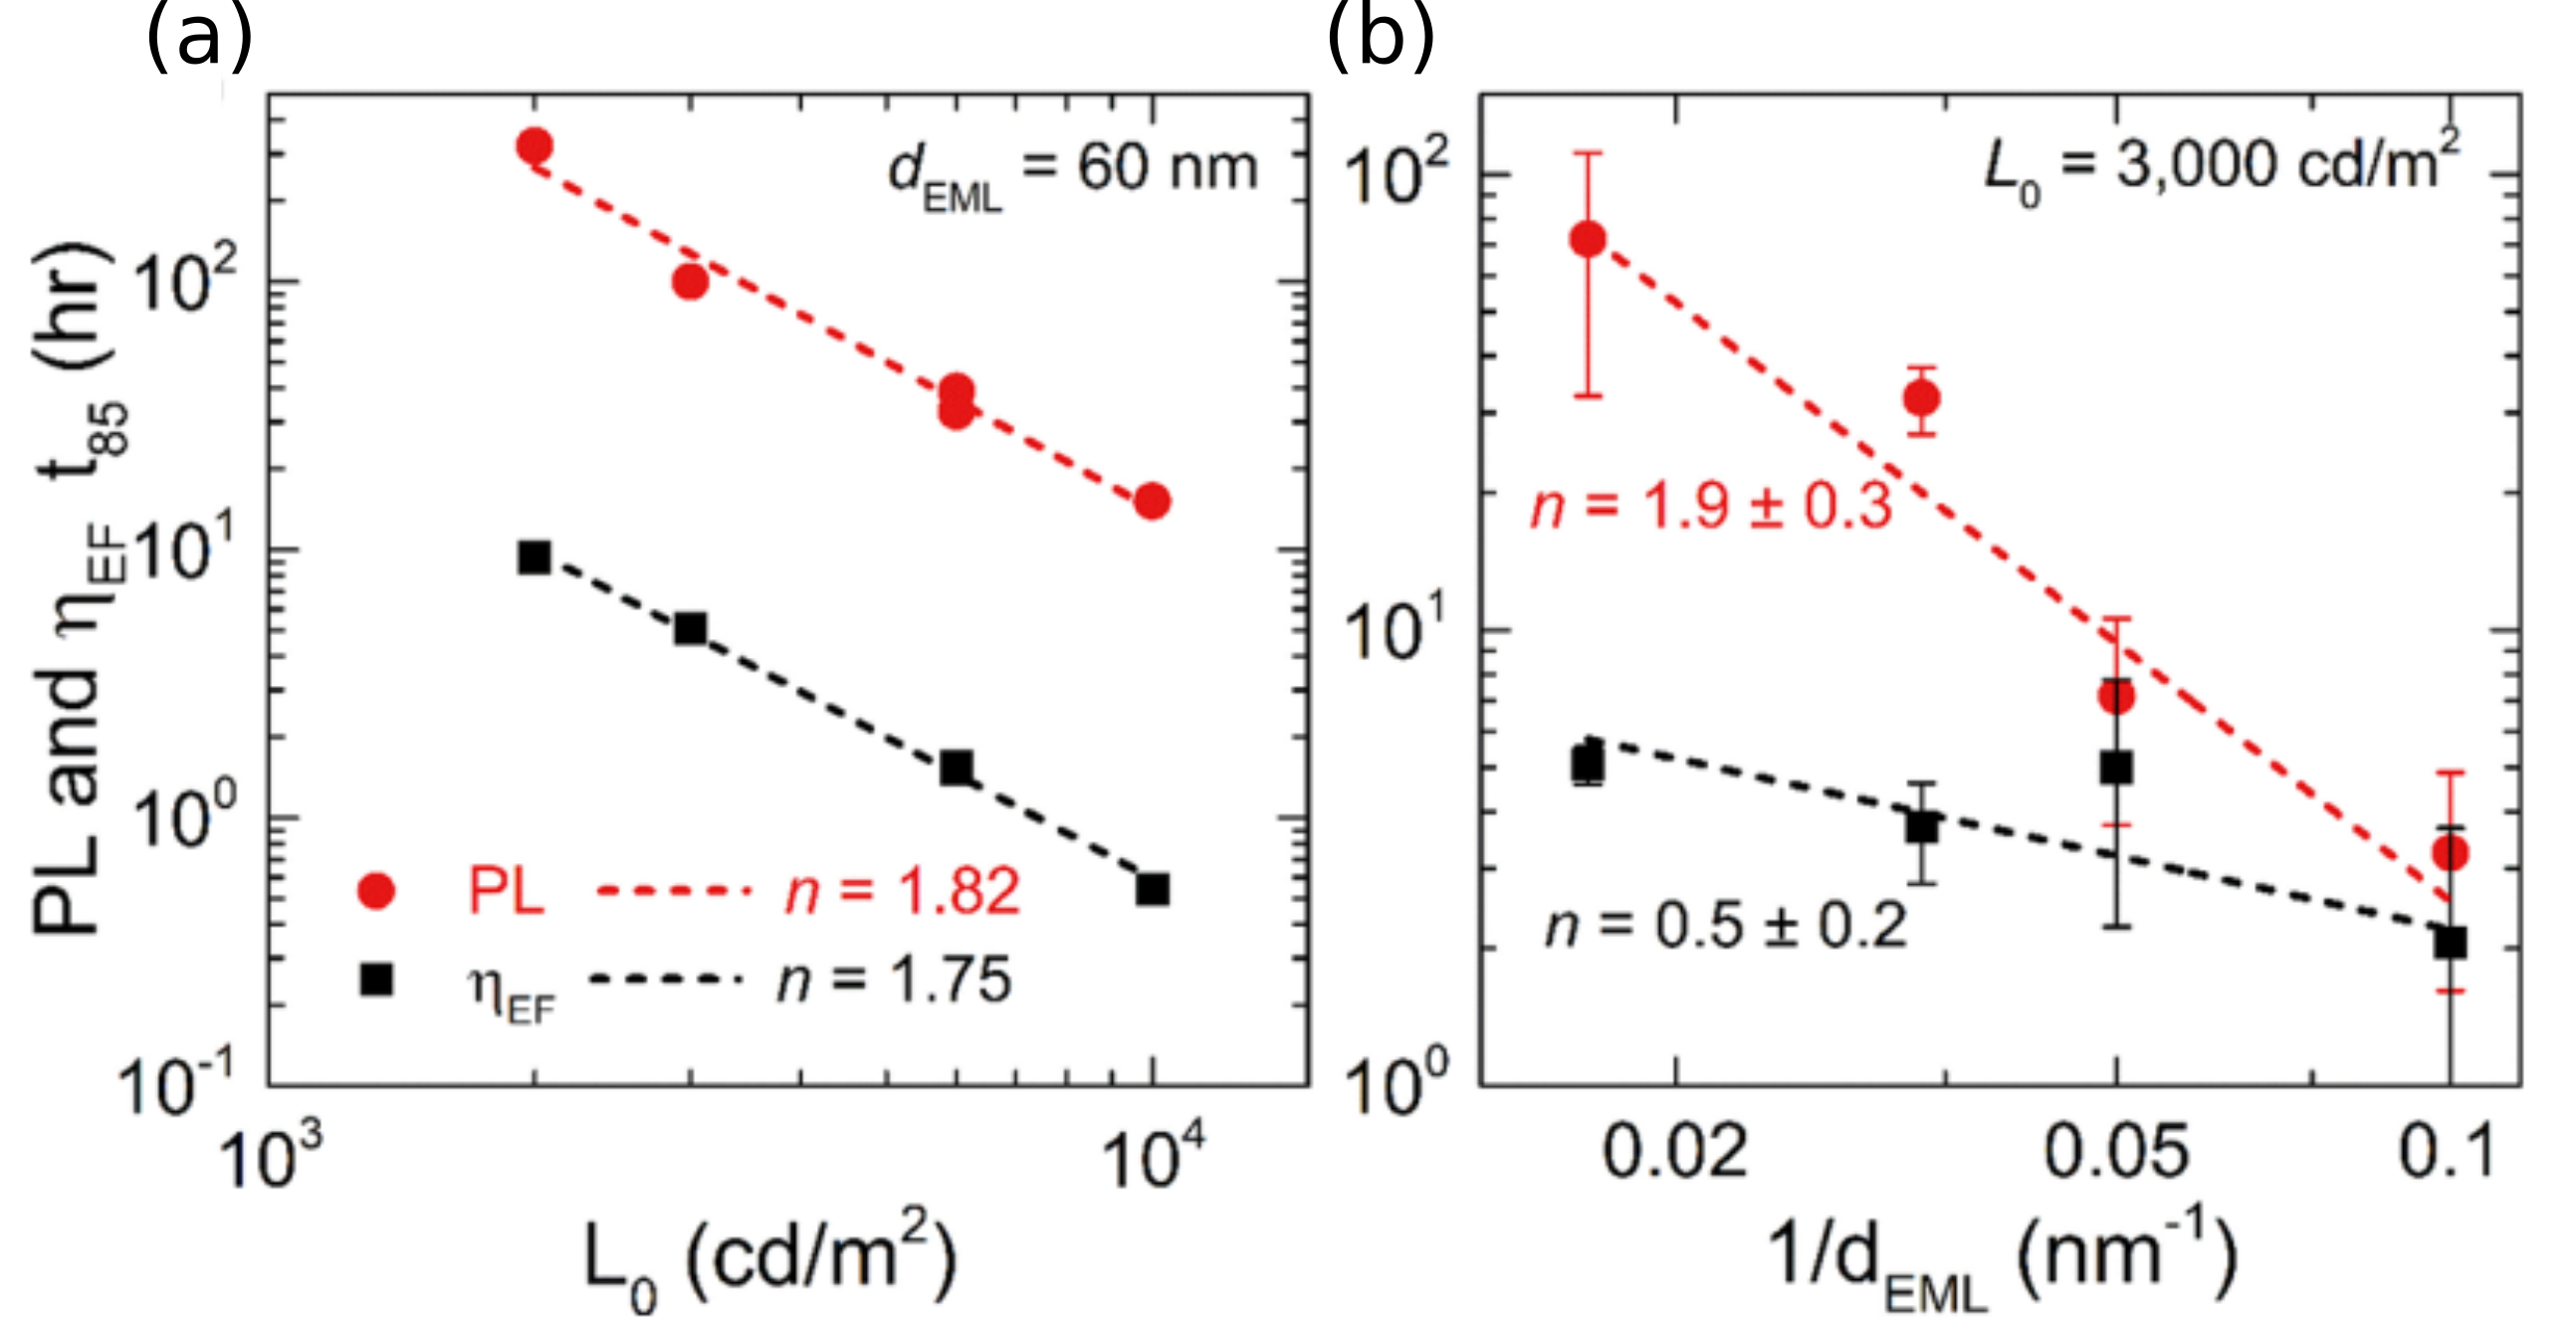
\includegraphics[width=.4\textwidth]{lifetimeApplications/meml_luminance}
\caption{Scaling behavior of \pl and \ef as a function of a) luminance and b) exciton density.}
\label{fig:meml_scaling}
\end{wrapfigure}


An alternative approach to investigating this connection is to look at the scaling relationships with luminance and exciton density.
OLED lifetime has been widely observed to follow a $1/L_0^n$ relationship,42 where $L_0$ is the initial luminance, and $n$ is a device specific parameter typically between 1-2. 
For these devices, $n = 1.8 \pm 0.1$ for the $t_{50}$ of EL and is independent of M-EML thickness. 
As shown in Figure \ref{fig:meml_scaling}a, the degradation in \pl and \ef for a 60 nm MEML show similar acceleration behavior as a function of luminance, with $n = 1.8$ and $n = 1.75$, respectively. 
Comparable slopes are seen for 10 nm and 30 nm M-EML devices. 

However, when scaled by $1/d_{EML}$, as displayed in Figure \ref{fig:meml_scaling}b, \ef and \pl show distinct scaling behavior. 
While PL $t_{85}$ shows a slope of $n = 1.9\pm0.3$, almost identical to the slope under luminance acceleration, \ef $t_{85}$ shows a much shallower slope of $n = 0.5\pm0.2$ (decreasing to $n = 0.3\pm0.3$ at 10,000 cd/m$^2$). 
This raises several important implications.
First, the identical slopes for PL provide further evidence that PL losses in this system are determined by the exciton density and the width of the recombination zone, and imply that there is a direct scaling law between recombination zone width and PL lifetime. 
While polaron density can play a role in PL degradation as well,27,43 it is unlikely that polaron density scales identically with both luminance and $d_{EML}$, implying that a single exciton driven or an exciton-exciton annihilation driven degradation mechanism is dominant in this system.

Second, the shallow dependence of \ef $t_{85}$ on RZ width (and hence exciton density) shown in Figure \ref{fig:meml_scaling}b suggests that excitons play a lesser role in \ef degradation. 
Notably, the difference in scaling with $L_0$ and $d_{EML}$ for \ef $t_{85}$ suggests that multiple degradation mechanisms comprise the total \ef loss.  
Exciton formation loss is often attributed to the accumulation of non-radiative recombination centers in the emissive layer,\supercite{Kondakov2003,Kondakov2007d} and has been linked to exciton-polaron interactions.\supercite{Zhang2017a}
The shallow dependence on RZ width (and hence exciton density) shown in Figure \ref{fig:meml_scaling}b suggests that the $d_{EML}$-dependent increase in \ef degradation to reflects the generation of non-radiative recombination centers by an exciton-mediated process, consistent with these reports. 
However, this mechanism alone cannot fully account for degradation in \ef, as the slope against initial luminancescaling with $L_0$ is much steeper (Figure \ref{fig:meml_scaling}a). 
This contrasting behavior suggests that a second mechanism which is independent of emissive layer exciton density governs \ef losses. 
This behavior is consistent with degradation mediated primarily by polarons or photodegradation of the cathode or anode interface, and may originate outside of the emissive layer. \supercite{Wang2012,Wang2010a}

These findings have implications for efforts in modeling OLED lifetime. 
Most modeling approaches assume that the same defect population responsible for exciton quenching was also responsible for non-radiative recombination of charge carriers. 
This immplies that the quenching population resides entirely in the emissive layer.2,7 \supercite{Giebink2008a,Zhang2014}
Defect populations external to the emissive layer have been considered, but only for the purposes of fitting voltage rise.45 \supercite{Lee2017}
In all cases, the generation of defects is proposed to proceed via bimolecular quenching processes.
While these treatments have yielded reasonable fits of the overall degradation behavior, they are unable to capture the behavior observed here.
Exciton formation and PL degradation would be expected to trend together within these formalisms, whereas Figure \ref{fig:meml_scaling} shows clearly distinct scaling behavior. 
Our results thus show that losses to \pl and \ef likely originate from kinetically distinct mechanisms.  
Moreover, the weak dependence of \ef on exciton density indicates and that degradation defects external to the emissive layer may play an important role in luminance loss, and should be considered in future modeling attempts.
Non-radiative recombination centers could have suitable energetics to serve as exciton quenchers, and vice versa.
However, because losses in \ef and \pl show different dependences with initial luminance and MEML thickness, the exciton quenchers formed in the EML are likely inefficient non-radiative recombination centers for charge carriers.

\subsection{Conclusion}

In conclusion, we find that broadening the recombination zone (RZ) sharply reduces the rate of PL degradation, showing a similar scaling relationship as with initial luminance variation. 
This confirms that PL degradation is strongly dependent on exciton density and has minimal dependence on changes in the polaron density as driven by the RZ.  
However, losses in the exciton formation efficiency (\ef) show a weaker dependence on RZ width, suggesting that \ef losses are less sensitive to exciton density and may partly originate outside of the M-EML in this system. 
Notably, the different dependences of PL and exciton formation efficiency loss on RZ width provide clear evidence that kinetically distinct pathways drive OLED degradation, and that a single degradation mechanism cannot be assumed when attempting to model device lifetime. 
These results highlight the capability of decoupled measurements of \pl and \ef losses to yield useful diagnostic insight into the source of device instability and shed light on the kinetics of degradation and the nature of defects.


\section{Dow Cohost}\label{sec:lifetime_dow}

\section{NPD Study}


\ifcsdef{mainfile}{}{\printbibliography}
\end{document}
